\documentclass[a4paper,14pt]{extarticle}
\usepackage[T1,T2A]{fontenc}
\usepackage[utf8]{inputenc}
\usepackage[english,russian,ukrainian]{babel}
\usepackage{minted}
\usepackage{geometry}
\usepackage{graphicx}
\usepackage{fontspec} 
\usepackage{dirtytalk}
\usepackage{amsmath}


\setmainfont{Liberation Serif}

\geometry{
    a4paper,
    left=20mm,
    top=20mm,
    right=10mm,
    bottom=20mm
}

\setlength{\emergencystretch}{2em}
\linespread{1.25}

\begin{document}
\begin{titlepage}
	\centering
    Міністерство освіти і науки України
    
    Харківський національний университет радіоелектроніки

    \vspace{1cm}
    Кафедра штучного інтелекту

    \vspace{2cm}
    Дисципліна: \say{Штучні нейронні мережі: архітектура}

    \vspace{2cm}
    \uppercase{лабораторна робота №1}

    
    % название лабораторной работы
    \uppercase{\say{ОЗНАЙОМЛЕННЯ З ВІЗУАЛЬНИМ
    СЕРЕДОВИЩЕМ ІМІТАЦІЙНОГО МОДЕЛЮВАННЯ MATLAB.
    СТВОРЕННЯ НЕЙРОННОЇ МЕРЕЖІ З ПРЯМОЇ
    ПЕРЕДАЧІ ІНФОРМАЦІЇ. АЛГОРИТМИ НАВЧАННЯ НЕЙРОННИХ МЕРЕЖ}}

    \vspace{4cm}
    \begin{minipage}[t]{10cm}
        Виконали ст. гр. ІТШІ-18-1:\\
        Апраксін Антон Романович\\
        Михно Євген Віталійович\\
        Соколенко Дмитро Олександрович
    \end{minipage}
    \hfill
    \begin{minipage}[t]{6cm}
        Прийняла:\\
        Чала О. С.\\
        з оцінкою \say{\rule{2cm}{0.15mm}}\\
        \say{\rule{0.7cm}{0.15mm}}\rule{2cm}{0.15mm}20\rule{0.7cm}{0.15mm}р
    \end{minipage}

	\vfill

	{Харків \the\year{}}
\end{titlepage}

\section*{Мета роботи}
Ознайомлення із візуальним середовищем імітаційного моделювання MATLAB
(Matrix laboratory). Освоєння методики створення нейронної мережі із прямою передачею даних. Освоєння різноманітних алгоритмів навчання нейронних мереж та
моделювання їх у середовищі MATLAB.

\section{Хід роботи}
\subsection{Оптимізатор GDM}
\inputminted[breaklines,linenos=true]{python}{gdm.py}

\subsubsection{Результати роботи GDM}
\inputminted[breaklines,linenos=true]{text}{output_gdm.txt}

\begin{figure}[H]
    \centering
    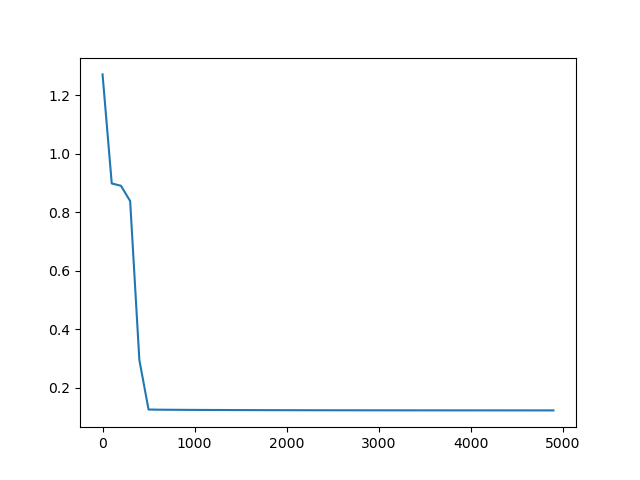
\includegraphics[width=0.75\textwidth]{gdm_loss.png}
    \caption{Графік помилки GDM}
\end{figure}
\begin{figure}[H]
    \centering
    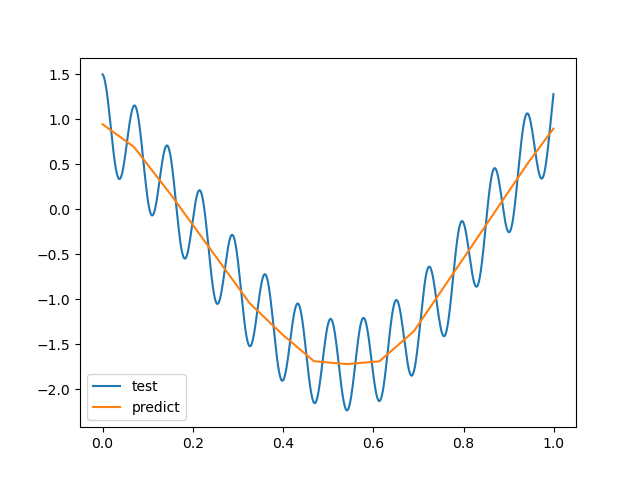
\includegraphics[width=0.75\textwidth]{gdm_func.png}
    \caption{Графік апроксимації функції оптимізатором GDM}
\end{figure}

\subsection{Оптимізатор CGF}
\inputminted[breaklines,linenos=true]{python}{cfg.py}

\subsubsection{Результати роботи CGF}
\inputminted[breaklines,linenos=true]{text}{output_cgf.txt}

\begin{figure}[H]
    \centering
    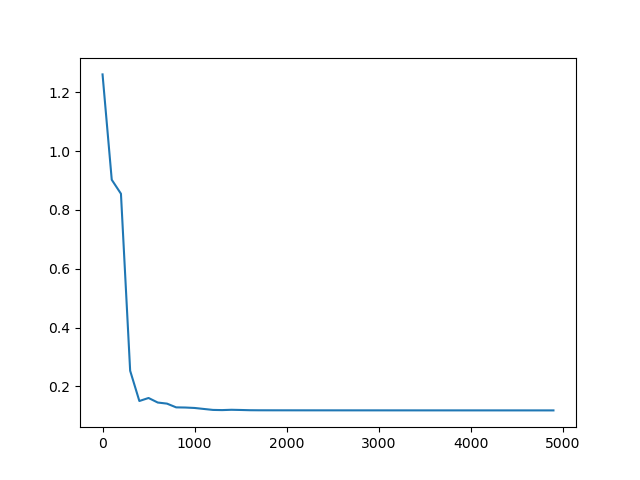
\includegraphics[width=0.75\textwidth]{cgf_loss.png}
    \caption{Графік помилки CGF}
\end{figure}
\begin{figure}[H]
    \centering
    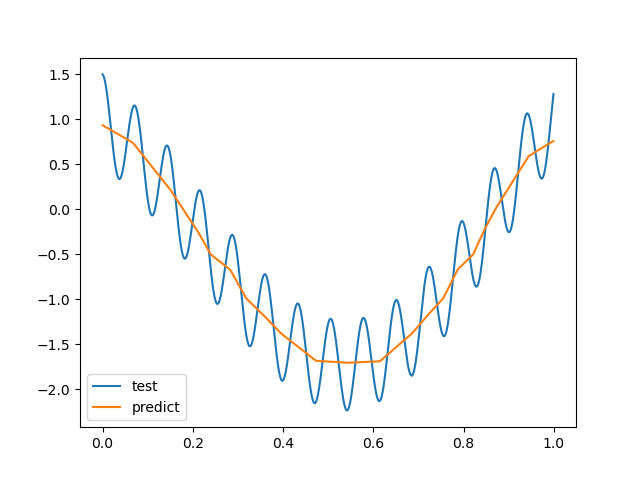
\includegraphics[width=0.75\textwidth]{cgf_func.png}
    \caption{Графік апроксимації функції оптимізатором CGF}
\end{figure}

\subsection{Оптимізатор BFGS}
\inputminted[breaklines,linenos=true]{python}{bfgs.py}

\subsubsection{Результати роботи BFGS}
\inputminted[breaklines,linenos=true]{text}{output_bfgs.txt}

\begin{figure}[H]
    \centering
    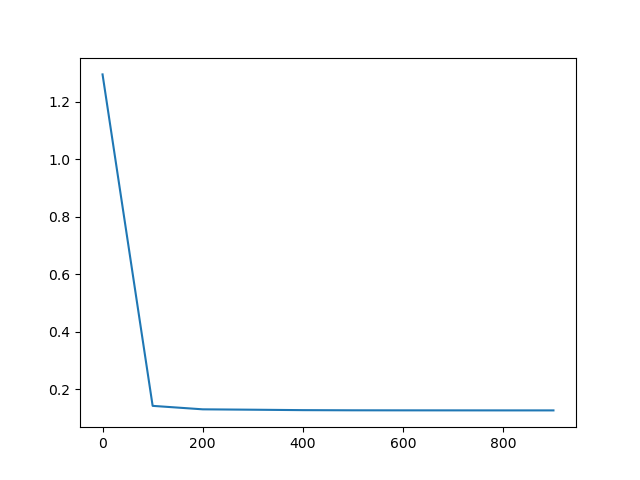
\includegraphics[width=0.75\textwidth]{bfgs_loss.png}
    \caption{Графік помилки BFGS}
\end{figure}
\begin{figure}[H]
    \centering
    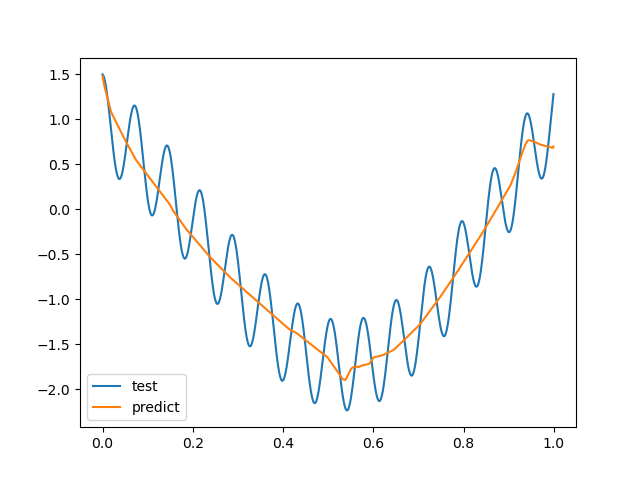
\includegraphics[width=0.75\textwidth]{bfgs_func.png}
    \caption{Графік апроксимації функції оптимізатором BFGS}
\end{figure}

\section*{Висновок}
В ході виконання лабораторної роботи ми ознайомилися із принципами створення нейронної мережі з прямою передачею інформації. За основу був взят код із
книжки The Neural Networks from Scratch. Нами були дописані необхідні алгоритми
оптимізації, що використовуються всередені мереж.

Алгоритм GDM показав найкращі результати щодо швидкості та точності виконання. BFGS є найповільнішим алгоритмом, але сходиться
за найменьшу кількість епох, проте складність реалізації
та досягнення такої самої точності, що і простіші алгоритми
робить його поганим алгоритмом для цієї задачі.

\end{document}

% \begin{figure}[H]
%     \centering
%     \includegraphics[width=0.75\textwidth]{rplot_iris.png}
%     \caption{Графік дерева вибірки Iris з дискретизацією через IG}
%     \label{fig:plot3}
% \end{figure}

% \begin{table}[H]
%     \centering
%     \begin{tabular}{ |c|c|c|c| } 
%      \hline
%      Мова   & \multicolumn{3}{c|}{Метод та датасет} \\ \hline
%             & Iris Thr. & Iris IG & SUSY \\ \hline
%      Python & 0.9333    & 0.9333  & 0.6799 \\ \hline
%      R      & 0.9333    & 0.9777  & 0.6594 \\ 
%      \hline
%     \end{tabular}
%     \caption{Порівняння точності класифікації}
%     \label{tab:t1}
% \end{table}
% \inputminted[breaklines,linenos=true]{scilab}{repl235.txt}
